\chapter{Fundamentals}
\section{First Section Name}
\lipsum[1-7]

\section{Second Section Name}
\subsection{Subsection Name}
\lipsum[1-4]

\subsubsection{It does not appear in contents}
\lipsum[1-2]

\section{Figures, Equations, Nomenclature and Reference}
\nomwithunits{R}{\(a,b,c\)}{half axes of ellipsoid}{\si{m}}%Example of nomenclature
\nomwithunits{G}{$\sigma$}{Surface Tension}{\si{F.m^{-2}}}%
\nomwithunits{R}{\(C\)}{dimensionless coefficient (e.g.\ for drag model)}{1}
\nomwithunits{G}{\( \varepsilon_0 \)}{vacuum permittivity}{\si{F.m^{-1}}}

To cite something in the text, you can use this \cite{Rumsey.2008} or this \cite{Virkus.2003, Warmkessel.1997}. Another citation is \cite{Rogow.2004}. Citavi can be used to generate a bibliography file for latex. An example of note\footnote{Ez Footnote}.  An example of equation can be seen in Eqn.~(\ref{eq:eq1}). Look at this multi-figures code in Fig.~(\ref{fig:fig1.1}) and Fig.~(\ref{fig:fig1.2}). And now a table in Tab.~(\ref{tab:tab1}). We have a bug, please do not reference a table before an equation environment. It COULD give problems. We are working on it.
\begin{equation}
\underbrace{C_{\s{1}} \ \rho_{\s{l}} \ v_{\s{b}}^2 \ d^{2}}_{F_\s{i}} \ + \underbrace{C_{\s{2}} \ \mu_{\s{l}} \ v_\s{b} \ d}_{F_\s{\mu}} \ = \ \underbrace {C_{\s{3}} \ \sigma \ d}_{F_\s{\sigma}} \ + \underbrace{C_{\s{4}} \ (\rho_\s{o} - \rho_\s{a}) \ g d^{3}}_{F_\s{b}}
\label{eq:eq1}
\end{equation} 
And another equation with a fraction can be seen in Eqn.~(\ref{eq:eq2})! Coooool! Microoo...\charmu m. 
\begin{equation}
v_\s{b}=C \ \myfrac[2pt]{1}{C_\s{D} \ Re} \ \myfrac[2pt]{(\rho_\s{O} - \rho_\s{a}) \ g}{\mu_\s{o}} \ d^2
\label{eq:eq2}
\end{equation}
\begin{figure}[h]
\begin{subfigure}{.5\textwidth}
  \centering
  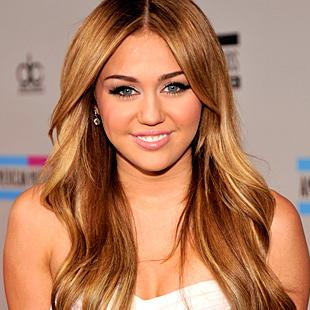
\includegraphics[width=.8\linewidth]{Graphics/vorher}
  \caption{vorher}
  \label{fig:fig1.1}
\end{subfigure}%
\begin{subfigure}{.5\textwidth}
  \centering
  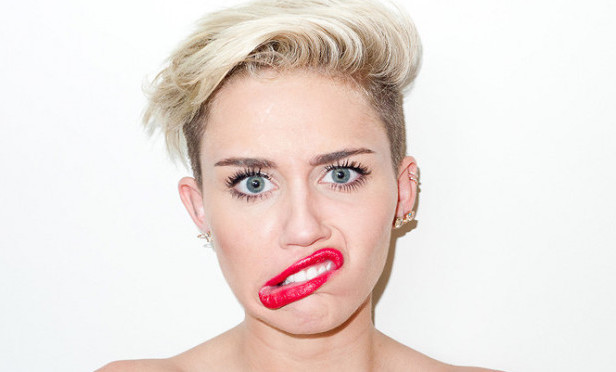
\includegraphics[width=.8\linewidth]{Graphics/nachher}
  \caption{nachher}
  \label{fig:fig1.2}
\end{subfigure}
\captionsetup{justification=raggedright,singlelinecheck=false}
\caption{plots of.... plots of.... plots of.... plots of.... plots of.... plots of.... plots of.... plots of.... plots of....}
\label{fig:fig}
\end{figure}
Nec vero habere virtutem satis est quasi artem aliquam nisi utare; etsi ars quidem cum ea non utare scientia tamen ipsa teneri potest, virtus in usu sui tota posita est; usus autem eius est maximus civitatis gubernatio, et earum ipsarum rerum quas isti in angulis personant, reapse non oratione perfectio. nihil enim dicitur a philosophis, quod quidem recte honesteque dicatur, quod ab iis partum confirmatumque sit, a quibus civitatibus iura discripta sunt. unde enim pietas, aut a quibus religio? unde ius aut gentium aut hoc ipsum civile quod dicitur? unde iustitia fides aequitas? unde pudor continentia fuga turpi<tu>dinis adpetentia laudis et honestatis? unde in laboribus et periculis fortitudo? nempe ab iis qui haec disciplinis informata alia moribus confirmarunt, sanxerunt autem alia legibus. 

\section{A section for tables}
An now another table in Tab.~(\ref{tab:tab2}). \\ \\ 
\begin{table*}[t] %t-top, b-bottom, h-in this place
  \centering
    \setlength\tabcolsep{1.5ex}
  \begin{tabular*}{\textwidth}{*{9}{c}}
    \hline \vspace{-2.5mm} \\
      & & && \multicolumn{2}{c}{ Schiller-Neumann }  && 
     \multicolumn{2}{c}{ ISO VG 46 } \\ \cline{5-6} \cline{8-9} \vspace{-2mm} \\ 
     \shortstack{$Q_\s{O}$ \\ $[l/min]$} & Design & \shortstack{$\alpha_\s{out}$ Exp \\ $[-]$} && \shortstack{$\alpha_\s{out}$ Sim \\ $[-]$} & \shortstack{Rel. Error \\ $[\%]$} && \shortstack{$\alpha_\s{out}$ Sim \\ $[-]$} & \shortstack{Rel. Error \\ $[\%]$} \vspace{1.5mm} \\
    \hline \vspace{-1.5mm} \\ 
    20 & 1. & 5.327E-4  && 8.347E-3 	& 990 	&& 7.661E-4 	& 44 \\
    30 & 1. & 1.236E-3  && 3.036E-2 	& 2260 	&& 1.286E-3 	& 4 \\
    50 & 1. & 2.368E-3  && 4.215E-2	    & 1542 	&& 2.567E-3 	& 8 \\
    70 & 1. & 4.746E-3  && 2.613E-2 	& 426 	&& 4.972E-3 	& 5 \\
    87 & 1. & 4.754E-3  && 2.280E-2 	& 347 	&& 5.097E-3 	& 7 \\
    70 & 2. & 1.416E-3  && 2.842E-3 	& 76.0 	&& 1.613E-3 	& 14 \\
    70 & 3. & 2.013E-3  && 1.241E-2 	& 440 	&& 2.297E-3 	& 14 \\
    70 & 4. & 1.228E-3  && 2.850E-3 	& 123 	&& 1.279E-3 	& 4 \\
    \hline
  \end{tabular*}
\captionsetup{justification=raggedright,singlelinecheck=false}
\caption{ Comparison of the drag correlations. Simulation results}
\label{tab:tab1}
\end{table*}
\lipsum[1-4]
\begin{table}[h]
\begin{center}
\setlength\tabcolsep{10ex}
\begin{tabular}{c c c}
%& & \\ % put some space after the caption
\hline
Name & Forces & Expression\\
\hline \\ [-4mm]
$\displaystyle Re$ & $\displaystyle \frac{F_\s{i}}{F_\s{\mu}}$  & $\displaystyle \frac{\rho_\s{O} v_\s{b} d}{\mu_\s{o}}$ \\ [2ex]
$\displaystyle Eo$ &  $\displaystyle \frac{F_\s{b}}{F_\s{\sigma}}$ & $\displaystyle \frac{(\rho_\s{o} - \rho_\s{A}) g d^2}{\sigma}$ \\[2ex]
$\displaystyle Mo$ & $\displaystyle \frac{F_\s{\mu}^4 F_\s{b}}{F_\s{\sigma}^3 F_\s{i}^2 }$ & $\displaystyle \frac{g \mu_\s{o}^4 (\rho_\s{o} - \rho_\s{a})}{\rho_\s{o}^2 \sigma^3}$ \\[2ex]
\hline
\end{tabular}
\end{center}
\captionsetup{justification=raggedright,singlelinecheck=false}
\caption{Dimensionless gruops}
\label{tab:tab2}
\end{table}



